%
% Sección de resultados de compraciones de desempeño.
% Artículo sobre tokenización.
%
% Proyecto Lovelace.
%

\section{Resultados y conclusiones}

En la tabla \ref{tabla:tiempos_tokenizacion} y la figura
\ref{figura:tiempos_unitarios} se muestran los resultados en tiempo de
las ejecuciones de los algoritmos presentados en secciones
anteriores\footnote{También se hizo la implementación de un DRBG como lo
describe el NIST en \cite{nist_aleatorios}}. Estos se llevaron a cabo en una
computadora con las siguientes características:

\begin{itemize}
  \item \textbf{Procesador:} Intel i5-7200U (2.5 GHz) de 4 núcleos.
  \item \textbf{Sistema operativo:} Arch Linux, kernel 4.17.
  \item \textbf{Base de datos:} MariaDB 10.1.
  \item \textbf{Compilador:} GCC 8.1.1
\end{itemize}

La comparación de los tiempos de tokenización y detokenización muestra como los
algoritmos reversibles son considerablemente más rápidos que los irreversibles.
Este resultado puede resultar un poco contraintuitivo, pues la generación de
tokens reversibles involucra más operaciones; es por esto que en la figura
\ref{figura:tiempos_tokenizacion} se muestran los tiempos de la generación de
tokens solamente, sin tomar en cuenta tiempos de acceso a base de datos.

Además de los tiempos de ejecución, también es importante señalar que los
irreversibles, al operar como funciones de un solo sentido, son un poco más
seguros que los reversibles: un atacante con acceso a la llave de cifrado puede
obtener el número de tarjeta correspondiente si se trata de un método
reversible, mientras que con un método irreversible necesita también acceso a la
base de datos.

\begin{table}
  %\tiny
  \centering
  \caption{Comparación de tiempos de tokenización.}
  \label{tabla:tiempos_tokenizacion}
  \begin{tabular}{c|c|c}
    \hline
    Algoritmo & Tokenización ($\mu$s) & Detokenización ($\mu$s) \\
    \hline
    FFX & 83 & 64 \\\hline 
BPS & 247 & 127 \\\hline 
TKR & 46260 & 373 \\\hline 
AHR & 3427 & 390 \\\hline 
DRBG & 54060 & 387 \\\hline 

  \end{tabular}
\end{table}

\begin{figure}[!t]
  \centering
  \subfloat[Tokenización y detokenización]{
    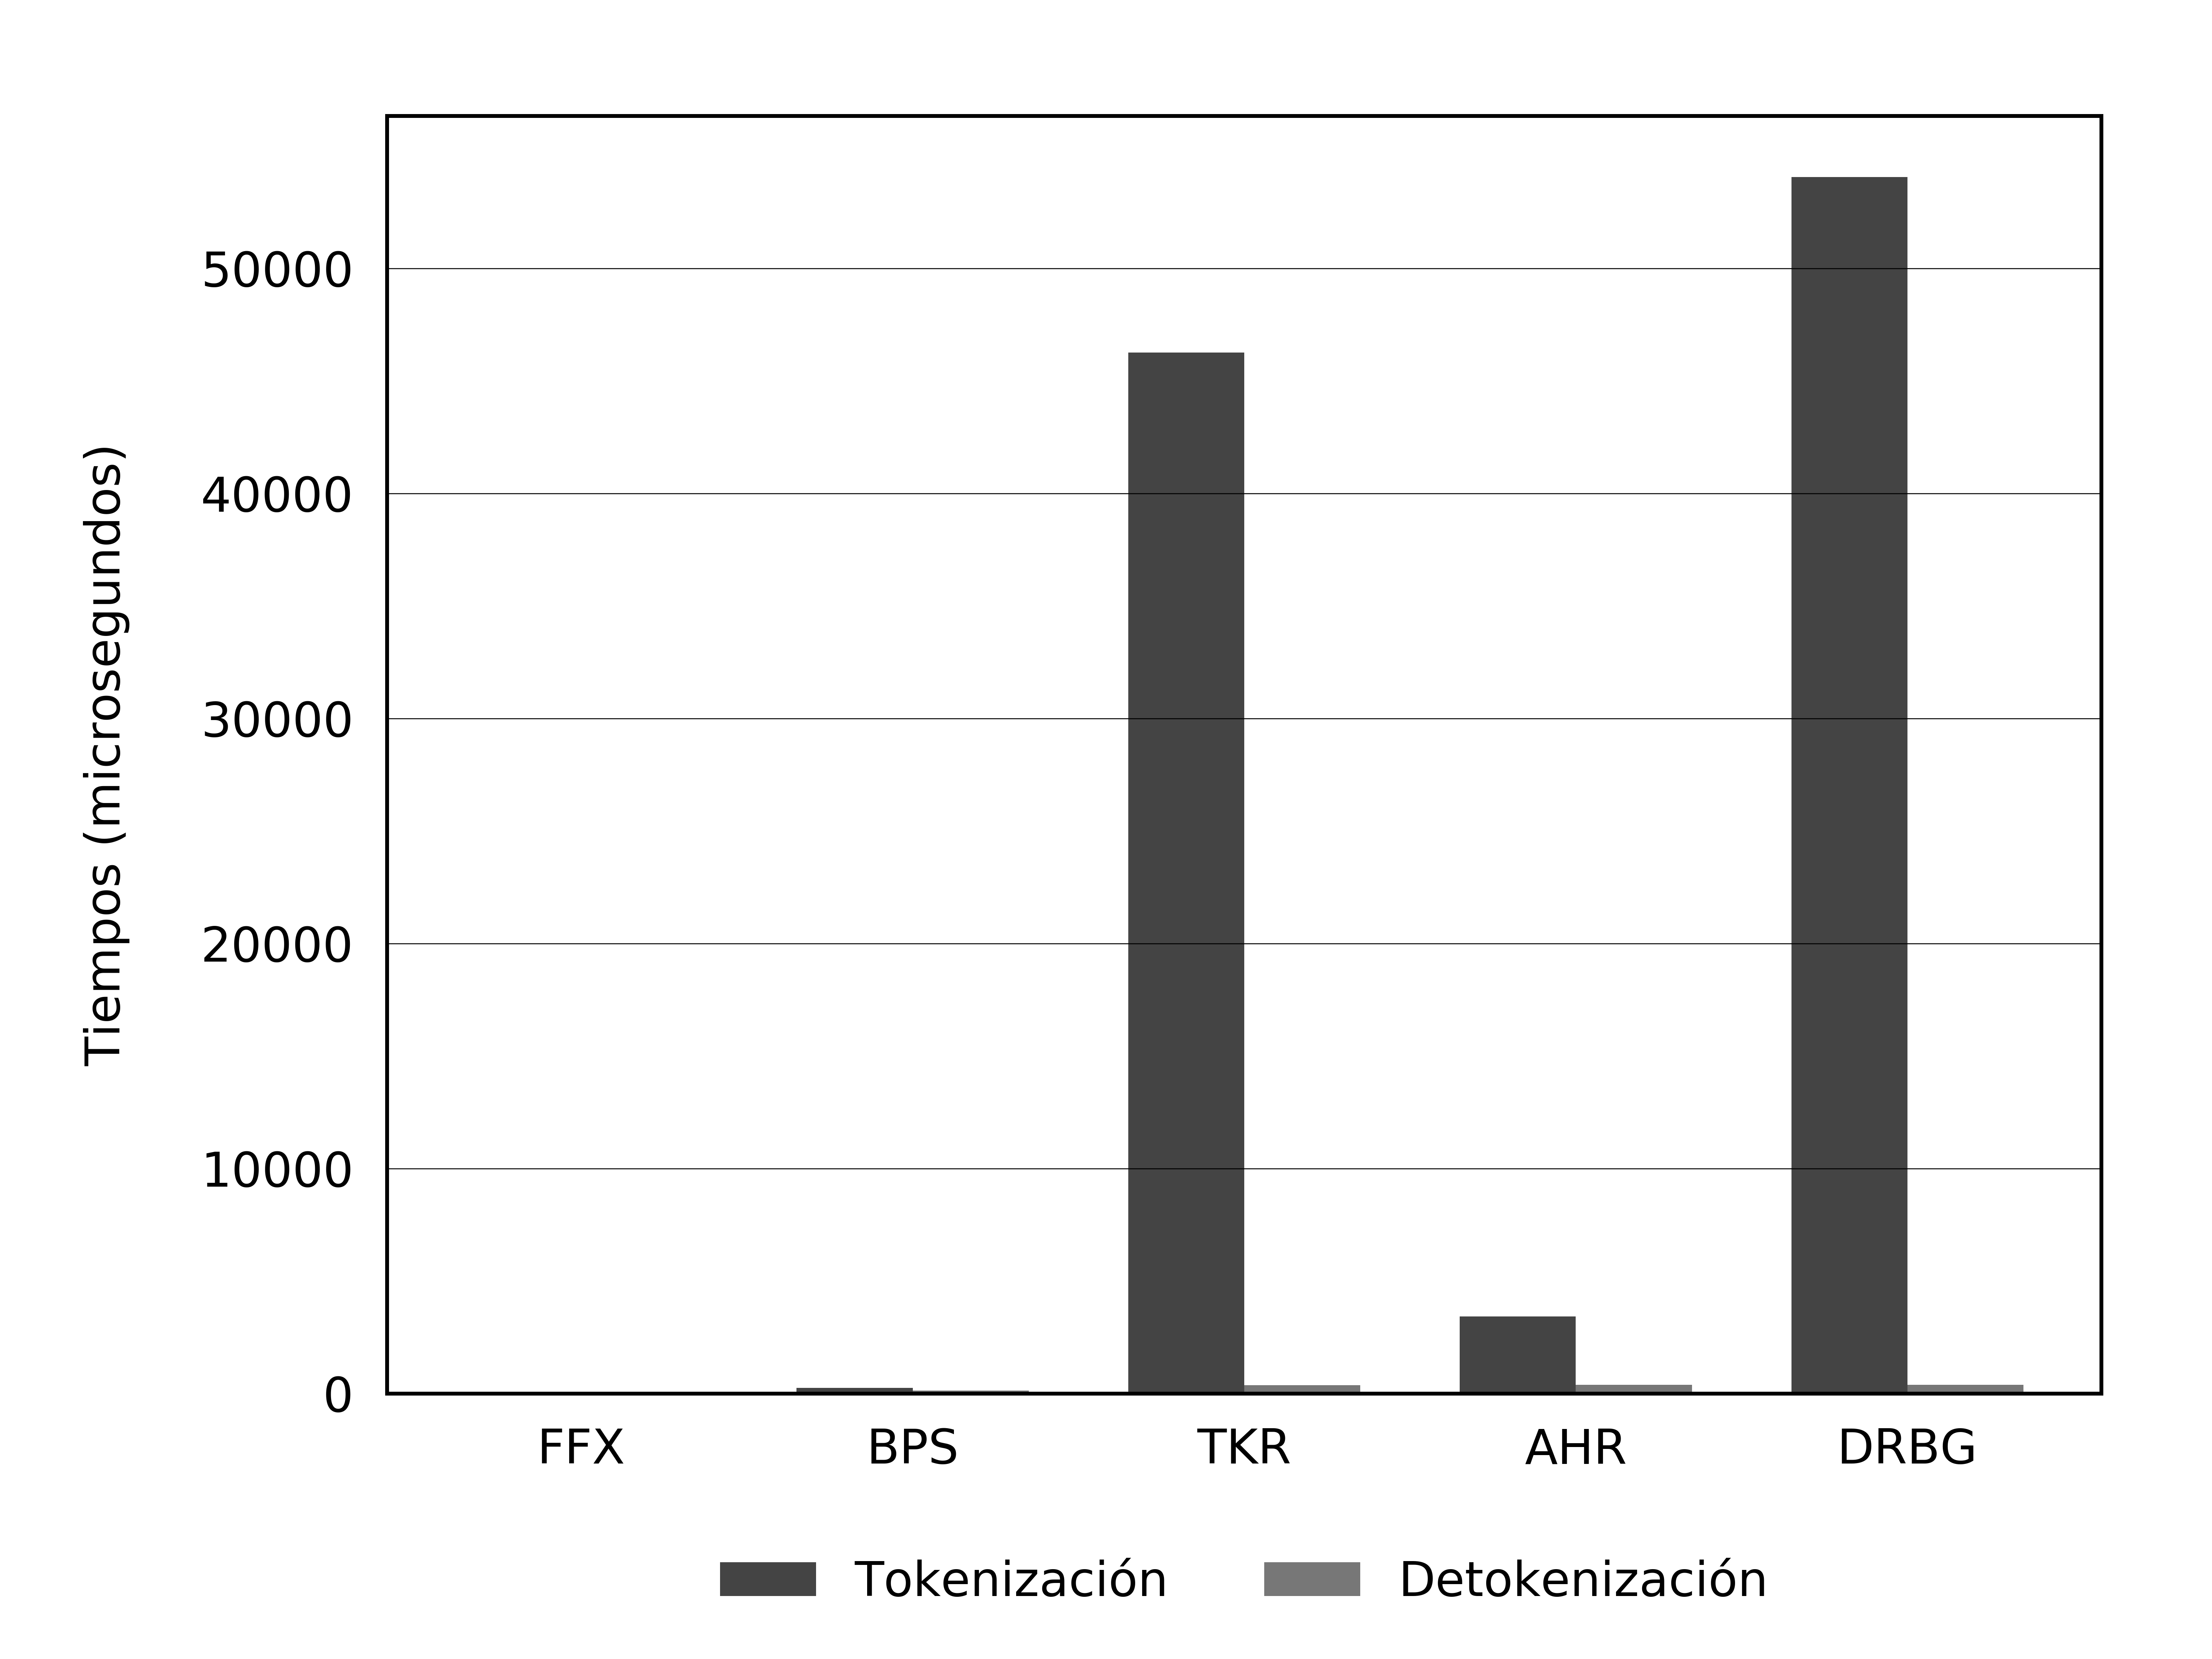
\includegraphics[width=1.62in]
      {../implementaciones/reportes/tiempos_unitarios.png}
    \label{figura:tiempos_unitarios}
  }
  \hfil
  \subfloat[Generación de tokens]{
    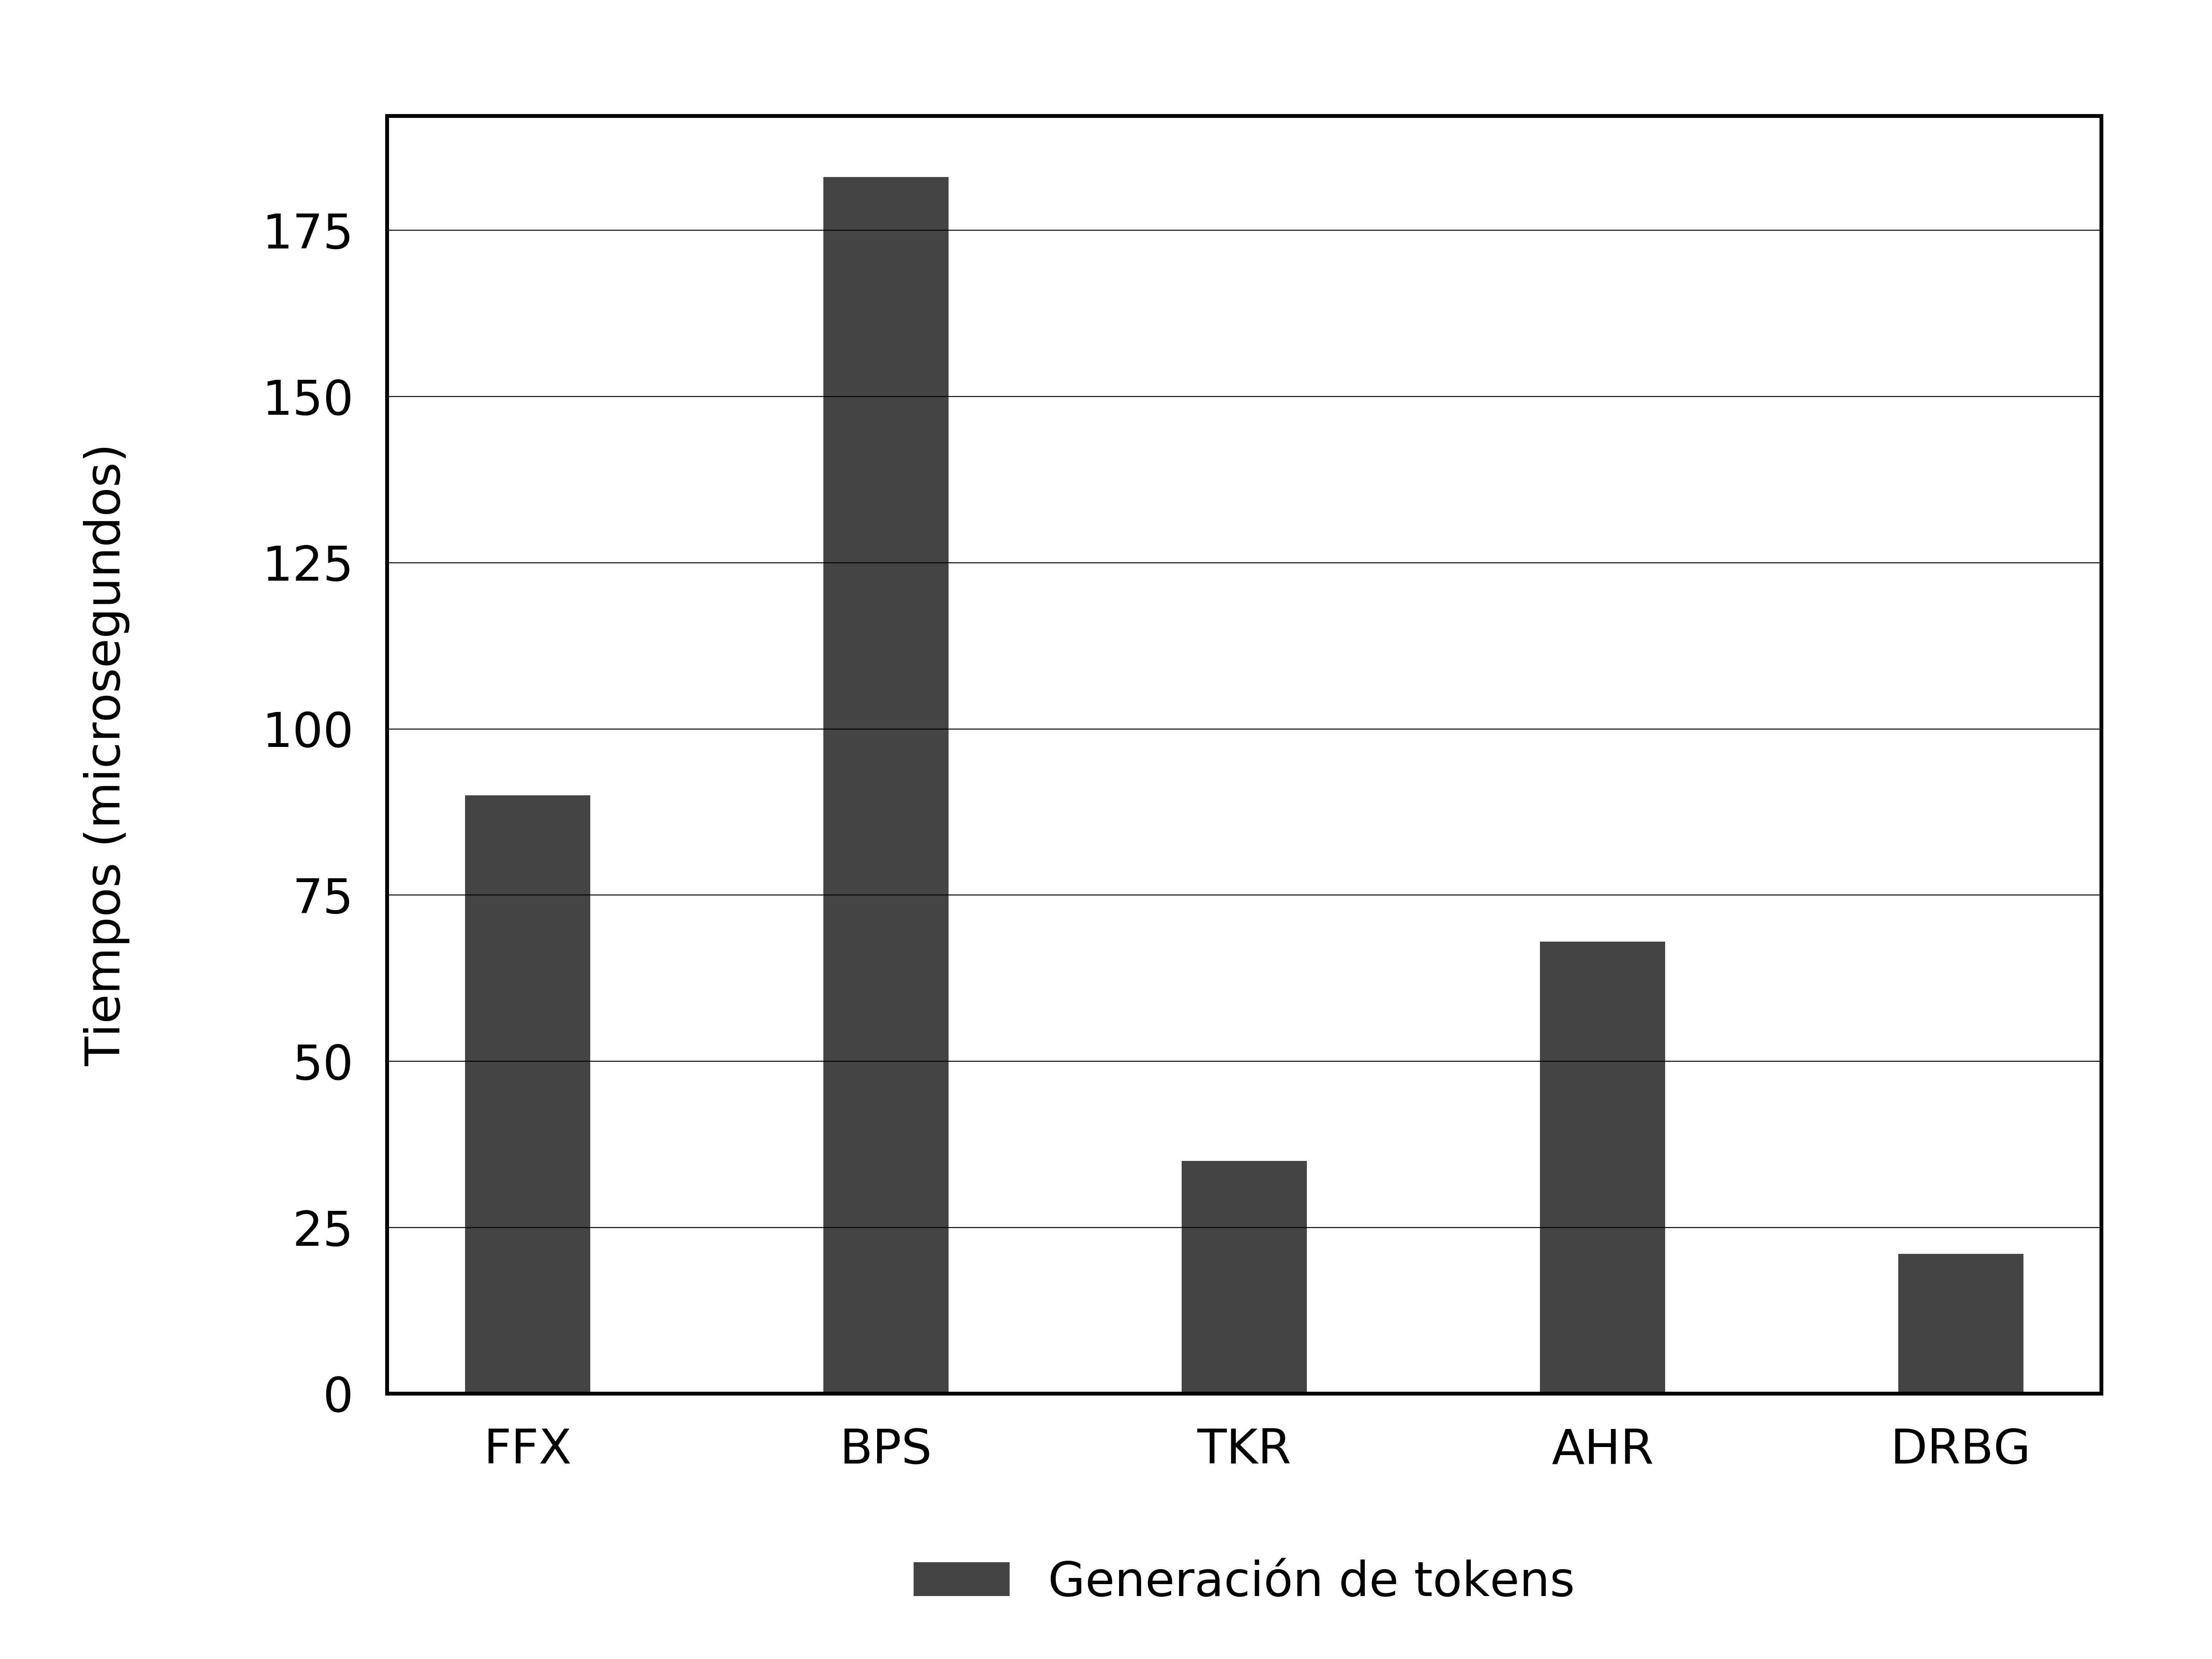
\includegraphics[width=1.62in]
      {../implementaciones/reportes/tiempos_tokenizacion.png}
    \label{figura:tiempos_tokenizacion}
  }
  \caption{Comparaciones de tiempos.}
  \label{fig_sim}
\end{figure}
